\documentclass[aspectratio=169]{ISAE-Beamer}
\usefonttheme[onlymath]{serif}
\usepackage{amsmath,amssymb,amsthm}
\usepackage{bm}
\usepackage{comment}
\usepackage{graphicx}
\usepackage{diffcoeff}
\usepackage{dsfont}
\usepackage{mathrsfs}
\usepackage[most]{tcolorbox}
\usepackage[caption=false]{subfig}

%\usepackage{multimedia}
\usepackage{media9}
\usepackage[backend=bibtex]{biblatex}

\graphicspath{{../Figures/}}

\definecolor{lightyellow}{RGB}{255, 255, 150}


\bibliography{bib_pres_IFACWC.bib}

\DeclareMathOperator{\Tr}{Tr}
\DeclareMathOperator*{\grad}{grad}
\DeclareMathOperator*{\Grad}{Grad}
\DeclareMathOperator*{\Div}{Div}
\renewcommand{\div}{\operatorname{div}}
\DeclareMathOperator*{\Hess}{Hess}

\DeclareMathOperator*{\argmax}{arg\,max}
\DeclareMathOperator*{\argmin}{arg\,min}

\def\onedot{$\mathsurround0pt\ldotp$}
\def\cddot{% two dots stacked vertically
	\mathbin{\vcenter{\baselineskip.67ex
			\hbox{\onedot}\hbox{\onedot}}%
}}

\renewcommand\bibfont{\scriptsize}


\makeatletter \renewcommand\d[1]{\ensuremath{%
		\;\mathrm{d}#1\@ifnextchar\d{\!}{}}}
\makeatother

\title[21st IFAC World Congress]{Partitioned finite element method for structured discretization with mixed boundary conditions}

\author[Andrea Brugnoli]{Andrea Brugnoli\inst{1}, Fl\'avio Luiz Cardoso-Ribeiro\inst{2}, Ghislain Haine\inst{1}, Paul Kotyczka\inst{3}}

\institute[ISAE]{\inst{1}ISAE-SUPAERO, France \and \inst{2}Instituto Tecnol\'ogico de Aeron\'autica, Brazil \and \inst{3}Technical University of Munich, Germany}

\date[29/5/20]{May, the 29th, 2020}

\AtBeginSection[]{
	\begin{frame}<beamer>
	\frametitle{Plan} %
	\tableofcontents[currentsection,subsectionstyle=shaded]  
\end{frame}
}

\AtBeginSubsection[]{
\begin{frame}<beamer>
\frametitle{Plan} %
\tableofcontents[currentsection,hideothersubsections,currentsubsection]  
\end{frame}
}

%\thanks{}

\begin{document}

\maketitle

\begin{frame}{Outline}

\tableofcontents

\end{frame}

\section{Introduction: problem statement}

\begin{frame}{Model description}
\begin{overlayarea}{\textwidth}{\textheight}
Model for the propagation of sound in air
\begin{equation*}
\diffp{}{t}
\begin{bmatrix}
\chi_s p \\
\mu_0 \bm{v} \\
\end{bmatrix} = -
\begin{bmatrix}
0 & \mathrm{div} \\
\mathrm{grad} & 0 \\
\end{bmatrix}
\begin{bmatrix}
p \\
\bm{v} \\
\end{bmatrix}, \qquad \text{on } \Omega = \{x \in [0, L],\; r \in [0, R],\; \theta = [0, 2 \pi)\}.
\end{equation*}
\only<1>{
\begin{itemize}
\item $p \in \mathbb{R}$  and $\bm{v} \in \mathbb{R}^3$: variations of pressure and velocity from a steady state;
\item $\mu_0$: the steady state mass density;
\item $\chi_s$: adiabatic compressibility factor;
\item $x, r, \theta$: axial, radial and tangential coordinates.
\end{itemize}
}
\only<2>{
\begin{columns}[T]
		\setlength{\abovedisplayskip}{3pt}
		\setlength{\belowdisplayskip}{3pt}
\begin{column}{.45\textwidth}
	Boundary conditions
	\begin{align*}
	p(x, R, \theta) &= - \mathcal{Z}(x, t) \, v_r(x, R, \theta), \\
	\bm{v} \cdot \bm{n}(0, r, \theta) &= -v_x(0, r, \theta) = - f(r), \\
	\bm{v} \cdot \bm{n}(L, r, \theta) &= +v_x(L, r, \theta) = + f(r), 
	\end{align*}
\end{column}
\begin{column}{.45\textwidth}
	Initial conditions
	\begin{equation*}
	\begin{aligned}
	p^0(x, r, \theta) &= 0, \\
	v_x^0(x, r, \theta) &= f(r), 
	\end{aligned}  \qquad
	\begin{aligned}
	v_r^0(x, r, \theta) &= g(r), \\
	v_\theta^0(x, r, \theta) &= 0.
	\end{aligned}    
	\end{equation*}
\end{column}
\end{columns}
\vspace{5pt}
The impedance $\mathcal{Z}$ and the axial $f(r)$ and radial flow $g(r)$ expressions are the following
\begin{equation*}
\begin{aligned}
\mathcal{Z}(x, t) = \mathds{1}\left\{ \frac{1}{3} L \leq \ x \ \leq \frac{2}{3} L, \,  t \geq 0.2 \ t_{\text{fin}} \right\} \mu_0 \, c_0, \\
f(r) = \left( 1 - \frac{r^2}{R^2} \right) v_0, \qquad
g(r) = 16 \frac{r^2}{R^4} \left( R - r \right)^2 v_0. 
\end{aligned}
\end{equation*}
}
\only<3>{
	\centering
	\vspace{2cm}
	\includegraphics[width=0.8\textwidth]{bc_3D_sketch.eps}	
}
\end{overlayarea}
\end{frame}



\begin{frame}{Model reduction by symmetry}
\begin{overlayarea}{\textwidth}{\textheight}
	
	Because of symmetry the model can be reduced to a 2D problem 
	\begin{equation*}
	\diffp{}{t}
	\begin{bmatrix}
	\chi_s p \\
	\mu_0 v_x \\
	\mu_0 v_r \\
	\end{bmatrix} = -
	\begin{bmatrix}
	0 & \partial_x & \partial_r + 1/r \\
	\partial_x & 0 & 0 \\
	\partial_r & 0 & 0 \\
	\end{bmatrix}
	\begin{bmatrix}
	p \\
	v_x \\
	v_r \\
	\end{bmatrix}, \quad \text{on } \Omega_{\text{r}} = \{x \in [0, L], r \in [0, R]\}.
	\end{equation*}
	\only<2>{
	The boundary conditions must now account for the symmetry condition at $r=0$
				\begin{align*}
				p(x, R, \theta) &= - \mathcal{Z}(x, t) \, v_r(x, R, \theta), \\
				\bm{v} \cdot \bm{n}(0, r, \theta) &= -v_x(0, r, \theta) = - f(r), \\
				\bm{v} \cdot \bm{n}(L, r, \theta) &= +v_x(L, r, \theta) = + f(r), \\
				\bm{v}\cdot \bm{n}(x, 0) &= v_r(x, 0) =0
				\end{align*}	
	}
\only<3>{
	\centering
	\includegraphics[width=0.7\textwidth]{bc_2D_sketch.eps}	
}
\end{overlayarea}
\end{frame}

\begin{frame}{A port-Hamiltonian structure}
\begin{overlayarea}{\textwidth}{\textheight}
	\setlength{\abovedisplayskip}{8pt}
	\setlength{\belowdisplayskip}{8pt}
The system can be rewritten compactly as a pH system in co-energy variables 
\begin{equation*}
\label{eq:sys_ph}
\mathcal{M} \partial_t{e} = \mathcal{J} e
\end{equation*}
where $\mathcal{M} = \mathrm{diag}([\chi_s, \ \mu_0, \ \mu_0])$  and $e = [e_p, \ \bm{e}_{v}]^\top= [p, \ \bm{v}]^\top$. \\
\vspace{8pt}
\only<1>{
The Hamiltonian is then computed as
\[
H = \frac{1}{2} \left(e, \mathcal{M} e  \right)_{\Omega_{\text{r}}}
\]
where $\left(\cdot, \cdot \right)_{\Omega_{\text{r}}}$ is the standard $L^2$ inner product in polar coordinates
\[
\left(\alpha, \beta \right)_{\Omega_{\text{r}}} = \int_{\Omega_{\text{r}}} \alpha \cdot \beta \ r \d{r} \d{x} = \int_{\Omega_{\text{r}}} \alpha \cdot \beta \ \d{\Omega_r}.
\]
The power flow is obtained by application of the Stokes theorem
\[
\dot{H} =  - \int_{0}^{L} \mathcal{Z}(x, t) v_r^2 \ R \d{x} \le 0 
\]
}
\only<2>{
The interconnection operator $\mathcal{J}$ can be decomposed into the sum of $\mathcal{J} = \mathcal{J}_{\text{div}} + \mathcal{J}_{\text{grad}}$
\begin{equation*}
\begin{aligned}
\mathcal{J}_{\text{div}} &= -\begin{bmatrix}
0 & \div_r \\
0 & 0 \\
\end{bmatrix}, \qquad \div_r = [\partial_x, \;   \partial_r + 1/r] \\
\mathcal{J}_{\text{grad}} &= -\begin{bmatrix}
0 & 0 \\
{\grad}_r & 0 \\
\end{bmatrix}, \qquad {\grad}_r =\begin{pmatrix}
\partial_x\\
\partial_r
\end{pmatrix}.
\end{aligned}
\end{equation*}
}
\end{overlayarea}
\end{frame}


\section{Finite dimensional discretization}

\begin{frame}{The partitioned finite element method (PFEM)}

\begin{block}{General procedure for PFEM}
	\setlength{\abovedisplayskip}{1pt}
	\setlength{\belowdisplayskip}{1pt}
	\begin{enumerate}
		\item Put the system into weak form:
		\begin{equation*}
		\left(v, \mathcal{M} \diffp{e}{t} \right)_{\Omega} = \left(v, \mathcal{J} e \right)_{\Omega}.
		\end{equation*}
		\item Apply integration by parts on a partition of $\mathcal{J}$:
		\begin{equation*}
		\left(v, \mathcal{J} e \right)_{\Omega} \overbrace{=}^{i.b.p.} j(v, e)_{\Omega} + b(v, u_\partial)_{\partial \Omega},
		\end{equation*}
		so that $j(v, e)_{\Omega}$ is a skew-symmetric bilinear form.
		\item Discretization by Galerkin method (same basis function for test and co-energy variables)
	\end{enumerate}
\end{block}
\end{frame}

\begin{frame}{Application to the wave equation}
\only<1>{
If the integration by parts is applied on $\mathcal{J}_{\text{div}}$
\begin{equation*}
\left(w, \mathcal{J} e \right)_{\Omega_{\text{r}}} = \left(\bm{w}_v, {\grad}_r e_p \right)_{\Omega_{\text{r}}} - \left({\grad}_r w_p, \bm{e}_v \right)_{\Omega_{\text{r}}} + \left(w_p, \textcolor{red}{u_N} \right)_{\partial \Omega_{\text{r}}}.
\end{equation*}
The skew-symmetric bilinear form 
\[ j_{\text{grad}}(w, e) := \left(\bm{w}_v, {\grad}_r e_p \right)_{\Omega_{\text{r}}} - \left({\grad}_r w_p, \bm{e}_v \right)_{\Omega_{\text{r}}} \]
is introduced, together with the boundary form
\begin{equation*}
\label{eq:f_N}
\left(w_p, \textcolor{red}{u_N} \right)_{\partial \Omega_{\text{r}}} = \int_{\partial \Omega_{\text{r}}} w_p \textcolor{red}{u_N} \ \d{\Gamma_r},
\end{equation*}
where $\textcolor{red}{u_N} = \bm{v} \cdot \bm{n} \vert_{\partial \Omega_r}$. The corresponding power conjugated output is given by $\textcolor{blue}{y_N} = p \vert_{\partial \Omega_r}$. \\
The system in weak form under Neumann boundary control is then written as
\begin{equation*}
\label{eq:wf_grad}
\begin{aligned}{}
(w, \mathcal{M} \partial_t{e})_{\Omega_{\text{r}}} &= j_{\text{grad}}(w, e) + \left(w_p, \textcolor{red}{u_N} \right)_{\partial \Omega_{\text{r}}}. \\
\left(w_N, \textcolor{blue}{y_N} \right)_{\partial \Omega_{\text{r}}} &= \left(w_N, p \right)_{\partial \Omega_{\text{r}}},
\end{aligned}
\end{equation*}
}


\only<2>{
If the integration by parts is carried out on $\mathcal{J}_{\text{grad}}$ 
\begin{equation*}
\left(w, \mathcal{J} e \right)_{\Omega_{\text{r}}} = \left(w_p, \div_r \bm{e}_v \right)_{\Omega_{\text{r}}} - \left(\div_r \bm{w}_v, e_p \right)_{\Omega_{\text{r}}} + \left(\bm{w}_v \cdot \bm{n}, \textcolor{blue}{u_D} \right)_{\partial \Omega_{\text{r}}}.
\end{equation*}
The skew-symmetric bilinear form 
\[ j_{\text{div}}(w, e) := \left(w_p, \div_r \bm{e}_v \right)_{\Omega_{\text{r}}} - \left(\div_r \bm{w}_v, e_p \right)_{\Omega_{\text{r}}} \]
is introduced, together with the boundary form
\begin{equation*}
\left(\bm{w}_v \cdot \bm{n}, \textcolor{blue}{u_D} \right)_{\partial \Omega_{\text{r}}} = \int_{\partial \Omega_{\text{r}}} \bm{w}_v \cdot \bm{n} \ \textcolor{blue}{u_D} \ \d{\Gamma_r}, 
\end{equation*}
where $\textcolor{blue}{u_D} = p \ \vert_{\partial \Omega_r}$. Adding  the conjugated output $\textcolor{red}{y_D} = \bm{v}\cdot~\bm{n}\vert_{\partial \Omega_r}$, the system in weak form under Dirichlet boundary control is then written as
\begin{equation*}
\label{eq:wf_div}
\begin{aligned}
(w, \mathcal{M} \partial_t{e})_{\Omega_{\text{r}}} &= j_{\text{div}}(w, e) + \left(\bm{w}_v \cdot \bm{n}, \textcolor{blue}{u_D} \right)_{\partial \Omega_{\text{r}}}, \\
\left(w_D, \textcolor{red}{y_D} \right)_{\partial \Omega_{\text{r}}} &= \left(w_D, \bm{v}\cdot\bm{n} \right)_{\partial \Omega_{\text{r}}},
\end{aligned}
\end{equation*}
}
\end{frame}

\begin{frame}{Mixed boundary condition}
To tackle mixed boundary conditions two approaches are developed:
\begin{itemize}
	\item a Lagrange multiplier based method;
	\item a virtual domain decomposition method.
\end{itemize} 	
\begin{figure}[b]%
	\centering
	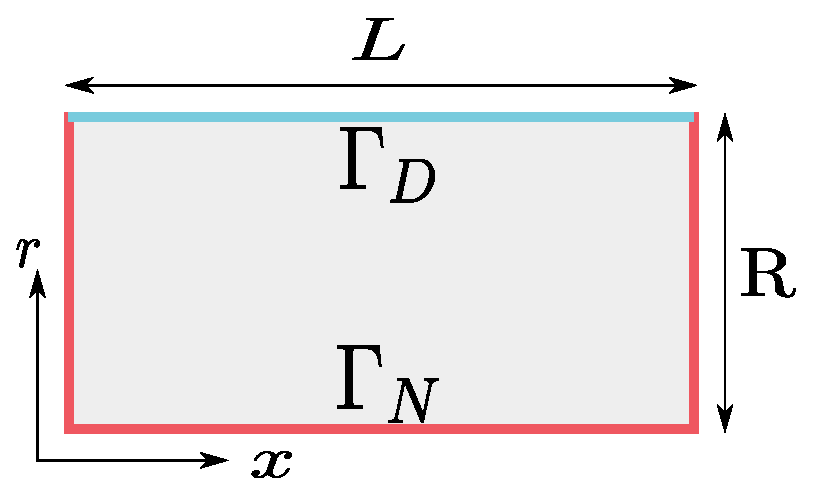
\includegraphics[width=0.4\columnwidth]{boundary_part.eps} \\
	\caption[bcpart]{Boundary partition for the problem.}
\end{figure}
\end{frame}


\subsection{Lagrange multiplier approach}

\begin{frame}{Weak form with Lagrange multipliers}
\setlength{\belowdisplayskip}{1pt}
\setlength{\abovedisplayskip}{1pt}
\begin{equation*}
\left(w, \mathcal{J} e \right)_{\Omega_{\text{r}}} =  j_{\text{grad}}(w, e) + \left(w_p, \bm{v}\cdot\bm{n}\vert_{\partial \Omega_{\text{r}}} \right)_{\partial \Omega_{\text{r}}}.
\end{equation*}
	The quantity $\bm{v}\cdot\bm{n}\vert_{\partial \Omega_{\text{r}}}$ is known on $\Gamma_N$ only. On $\Gamma_D$ the Lagrange multiplier $\lambda_D$ is introduced 
	\begin{equation*}
	\label{eq:bdint_dae}
	\int_{\partial \Omega_{\text{r}}} w_p \bm{v} \cdot \bm{n} \d{\Gamma_r} = \int_{\Gamma_N} w_p u_N \ \d{\Gamma_r} + \int_{\Gamma_D} w_p \lambda_D \d{\Gamma_r}.
	\end{equation*}
	The constraint  is the non-homogeneous Dirichlet condition
	\begin{equation*}
	\label{eq:wf_con}
	\int_{\Gamma_D} w_\lambda (p - u_D) \d{\Gamma_r} = 0, \qquad \text{$w_\lambda$ test function for the Lagrange multiplier.}
	\end{equation*}
	
	\begin{exampleblock}{Final Weak Form with Lagrange multiplier}
	\begin{equation*}
	\begin{aligned}
	m(w, \partial_t{e}) &= j_{\text{grad}}(w, e) + \left(w_p, \lambda_D \right)_{\Gamma_D} + \left(w_p, \textcolor{red}{u_N} \right)_{\Gamma_N}, \\
	0 &= - \left(w_\lambda, p \right)_{\Gamma_D} + \left(w_\lambda, \textcolor{blue}{u_D} \right)_{\Gamma_D}, \\
	\left(w_N, \textcolor{blue}{y_N} \right)_{\Gamma_N} &= \left(w_N, p \right)_{\Gamma_N}, \\
	\left(w_D, \textcolor{red}{y_D} \right)_{\Gamma_D} &= \left(w_D, \lambda_D \right)_{\Gamma_D}, 
	\end{aligned}
	\end{equation*}
	\end{exampleblock}


\end{frame}

\begin{frame}
	A Galerkin method can now be applied to retrieve a finite dimensional pH system. This means that corresponding test and trial functions are discretized using the same basis
	\begin{equation*}
	\label{eq:basis_func}
	\begin{aligned}
	\begin{aligned}
	p &\approx \sum_{i=1}^{n_p} \phi_p^i(x, r) p^i, \\
	\bm{v} &\approx \sum_{i=1}^{n_v} \bm\phi_v^i(x, r) v^i, \\
	\end{aligned} \quad
	\begin{aligned}
	*_D &\approx \sum_{i=1}^{n_D} \phi^i_\Gamma(s_D) *^i_D, \quad s_D \in \Gamma_D, \quad (* = \{u, y, \lambda\}), \\
	*_N &\approx \sum_{i=1}^{n_N} \phi_\Gamma^i(s_N) *^i_N, \quad s_N \in \Gamma_N, \quad (* = \{u,  y\}).
	\end{aligned} 
	\end{aligned}
	\end{equation*}
	A pHDAE system is obtained:
	\begin{equation*}
	\begin{aligned}
	\label{eq:discr_phdae}
	\begin{bmatrix}
	\mathbf{M} & \mathbf{0} \\
	\mathbf{0} & \mathbf{0} \\
	\end{bmatrix} \frac{\d}{\d t}
	\begin{pmatrix}
	\mathbf{e}\\
	\bm{\lambda}_D \\
	\end{pmatrix}
	&= \begin{bmatrix}
	\mathbf{J} & \mathbf{G}_D\\
	-\mathbf{G}_D^\top & \mathbf{0} \\
	\end{bmatrix}
	\begin{pmatrix}
	\mathbf{e}\\
	\bm{\lambda}_D \\
	\end{pmatrix} + \begin{bmatrix}
	\mathbf{B}_N & \mathbf{0}\\
	\mathbf{0} & \mathbf{B}_D \\
	\end{bmatrix}
	\begin{pmatrix}
	\textcolor{red}{\mathbf{u}_N} \\
	\textcolor{blue}{\mathbf{u}_D} \\
	\end{pmatrix}, \\
	\begin{bmatrix}
	\mathbf{M}_{\Gamma_N} & \mathbf{0} \\
	\mathbf{0} & \mathbf{M}_{\Gamma_D} \\
	\end{bmatrix}
	\begin{pmatrix}
	\textcolor{blue}{\mathbf{y}_N} \\
	\textcolor{red}{\mathbf{y}_D} \\
	\end{pmatrix} &=
	\begin{bmatrix}
	\mathbf{B}_N^\top & \mathbf{0} \\ 
	\mathbf{0} & \mathbf{B}_D^\top \\ 
	\end{bmatrix}
	\begin{pmatrix}
	\mathbf{e}\\
	\bm{\lambda}_D \\
	\end{pmatrix}.
	\end{aligned}
	\end{equation*}
	
\end{frame}

\begin{frame}{Imposition of the boundary conditions}
	Take the weak form of $u_D=-\mathcal{Z}\lambda_D=-\mathcal{Z}y_D$:
	\[ \mathbf{M}_{\Gamma_D} \textcolor{blue}{\mathbf{u}_D} = - \mathbf{M}_{\Gamma_D, \mathcal{Z}} \textcolor{red}{\mathbf{y}_D},
	\]
	This amounts to applying the control law
	\[ \mathbf{u}_D  = -\mathbf{Z} \mathbf{B}_D^T \bm{\lambda}_D, \qquad \mathbf{Z} = \mathbf{M}_{\Gamma_D}^{-1} \mathbf{M}_{\Gamma_D, \mathcal{Z}} \mathbf{M}_{\Gamma_D}^{-1}
	\]
	The Neumann boundary condition is imposed projecting $u_N = f(r)$. 
	\begin{block}{Finite dimensional system with Lagrange multiplier}
	\begin{equation*}
	\label{eq:sys_dae}
	\begin{bmatrix}
	\mathbf{M} & \mathbf{0} \\
	\mathbf{0} & \mathbf{0} \\
	\end{bmatrix} \frac{\d}{\d t}
	\begin{bmatrix}
	\mathbf{e}\\
	\bm{\lambda}_D \\
	\end{bmatrix}
	= \begin{bmatrix}
	\mathbf{J} & \mathbf{G}_D\\
	-\mathbf{G}_D^\top & -\mathbf{R} \\
	\end{bmatrix}
	\begin{bmatrix}
	\mathbf{e}\\
	\bm{\lambda}_D \\
	\end{bmatrix} + \begin{bmatrix}
	\mathbf{b}_N \\
	\mathbf{0} \\
	\end{bmatrix},
	\end{equation*}
	with $\mathbf{R} = \mathbf{B}_D \mathbf{Z} \mathbf{B}_D^T$ a symmetric positive definite matrix. 
	\end{block}
	
\end{frame}

\subsection{Virtual domain decomposition}

\begin{frame}{Decomposition of the domain}
First of all the domain has to be decomposed. \\

The interface between the two subdomain is chosen to get regular meshes on both subdomains.
\begin{figure}[t]%
	\centering
	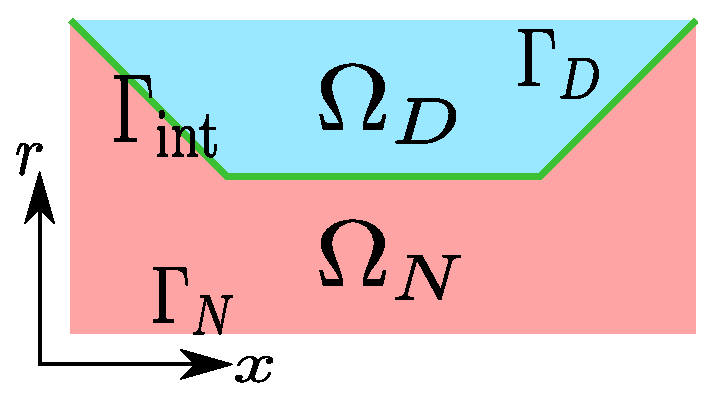
\includegraphics[width=0.5\columnwidth]{domain_split.eps} \\
	\caption{Virtual decomposition of the domain.}
\end{figure}
\end{frame}

\begin{frame}
	Two weak formulations are constructed: 
	\begin{align*}
	\left(w, \mathcal{M} \partial_t{e} \right)_{\Omega_N} &= \left(w, \mathcal{J} e \right)_{\Omega_{N}}, \qquad \text{where } \left(\alpha, \beta \right)_{\Omega_N} = \int_{\Omega_{N}} \alpha \cdot \beta \d{\Omega_{N}}, \\
	\left(w, \mathcal{M} \partial_t{e} \right)_{\Omega_D} &= \left(w, \mathcal{J} e \right)_{\Omega_{D}}, \qquad \text{where } \left(\alpha, \beta \right)_{\Omega_D} = \int_{\Omega_{D}} \alpha \cdot \beta \d{\Omega_{D}}.
	\end{align*}
	The integration by parts is performed differently on each subdomain to highlight the appropriate boundary input
	\begin{equation*}
	\begin{aligned}
	\left(w, \mathcal{M} e \right)_{\Omega_{N}} &= j_{\text{grad}}^{\Omega_N}(w, e) + \left(w_p, \textcolor{red}{u_N} \right)_{\partial \Omega_N}, \\
	\left(w, \mathcal{M} e \right)_{\Omega_{D}} &= j_{\text{div}}^{\Omega_D}(w, e) + \left(\bm{w}_v \cdot \bm{n}, \textcolor{blue}{u_D} \right)_{\partial \Omega_D},  \\
	\end{aligned} 
	\end{equation*}
where the bilinear skew-symmetric forms are defined on each subdomain
\begin{equation*}
	\begin{aligned}
	j_{\text{grad}}^{\Omega_{N}}(w, e) &:= \left(\bm{w}_v, {\grad}_r e_p \right)_{\Omega_{N}} - \left({\grad}_r w_p, \bm{e}_v \right)_{\Omega_{N}}, \\
	j_{\text{div}}^{\Omega_{D}}(w, e) &:= \left(w_p, \div_r \bm{e}_v \right)_{\Omega_{D}} - \left(\div_r \bm{w}_v, e_p \right)_{\Omega_{D}}.
	\end{aligned}
\end{equation*}
\end{frame}

\begin{frame}
The boundary terms are then split into two contributions
\begin{equation*}
\begin{aligned}
\partial\Omega_N = \Gamma_N \cup \Gamma_{\text{int}} &\implies \\
\partial\Omega_D = \Gamma_D \cup \Gamma_{\text{int}} &\implies
\end{aligned}
\begin{aligned}
\left(w_p, \textcolor{red}{u_N} \right)_{\partial \Omega_N} &= \left(w_p, \textcolor{red}{u_N} \right)_{\Gamma_N} + \left(w_p, \textcolor{red}{u_N}\right)_{\Gamma_{\text{int}}}, \\
\left(\bm{w}_v \cdot \bm{n}, \textcolor{blue}{u_D} \right)_{\partial \Omega_D} &= \left(\bm{w}_v \cdot \bm{n}, \textcolor{blue}{u_D} \right)_{\Gamma_D} + \left(\bm{w}_v \cdot \bm{n}, \textcolor{blue}{u_D} \right)_{\Gamma_{\text{int}}}.
\end{aligned}
\end{equation*}

Two finite dimensional pH systems are obtained

\begin{tcbraster}[raster columns=2, raster equal height]
	\begin{tcolorbox}[width=0.48\textwidth, nobeforeafter, colframe=red,title=Subdomain $\Omega_N$,  coltitle=black]%%
		\begin{equation*}
		\begin{aligned}
		\mathbf{M}_N {\dot{\mathbf{e}}_N} &= \mathbf{J}_N \mathbf{e}_N  + \mathbf{B}_N \textcolor{red}{\mathbf{u}_N} + \mathbf{B}_{N}^{\text{int}} \textcolor{red}{\mathbf{u}_N^{\text{int}}}, \\
		\mathbf{M}_{\Gamma_N} \textcolor{blue}{\mathbf{y}_N} &= \mathbf{B}_{N}^\top \mathbf{e}_N, \\
		\mathbf{M}_{\Gamma_{\text{int}}} \textcolor{blue}{\mathbf{y}_N^{\text{int}}} &=  \mathbf{B}_{N}^{\text{int}\, \top} \mathbf{e}_N, \\
		\end{aligned}
		\end{equation*}
		with Hamiltonian $H_{d, N} = \frac{1}{2} {\mathbf{e}}_{N}^\top \mathbf{M}_N {{\mathbf{e}}_N}$
	\end{tcolorbox} 
	\begin{tcolorbox}[width=0.48\textwidth, nobeforeafter,  colframe=cyan,title=Subdomain $\Omega_D$, coltitle=black]%%
		\begin{equation*}
		\begin{aligned}
		\mathbf{M}_D \dot{\mathbf{e}}_D &= \mathbf{J}_D \mathbf{e}_D + \mathbf{B}_D \textcolor{blue}{\mathbf{u}_D} + \mathbf{B}_{D}^{\text{int}} \textcolor{blue}{\mathbf{u}_D^{\text{int}}}, \\
		\mathbf{M}_{\Gamma_D} \textcolor{red}{\mathbf{y}_D} &= \mathbf{B}_{D}^\top \, \mathbf{e}_D, \\
		\mathbf{M}_{\Gamma_{\text{int}}} \textcolor{red}{\mathbf{y}_D^{\text{int}}} &= \mathbf{B}_{D}^{\text{int}\, \top} \mathbf{e}_D. \\
		\end{aligned}
		\end{equation*}
		with Hamiltonian $H_{d, D} = \frac{1}{2} {\mathbf{e}}_{D}^\top \mathbf{M}_D {{\mathbf{e}}_D}$
	\end{tcolorbox}
\end{tcbraster}
\end{frame}


\begin{frame}{Power preserving interconnection}
A gyrator interconnection is performed
\begin{equation*}
\textcolor{red}{\mathbf{u}_N^{\text{int}}} = - \textcolor{red}{{\mathbf{y}}_D^{\text{int}}} = - \mathbf{M}_{\Gamma_{\text{int}}}^{-1}\mathbf{B}_{D}^{\text{int}\, \top} \mathbf{e}_D, \qquad
\textcolor{blue}{\mathbf{u}_D^{\text{int}}} = \textcolor{blue}{\mathbf{y}_N^{\text{int}}} = \mathbf{M}_{\Gamma_{\text{int}}}^{-1} \mathbf{B}_{N}^{\text{int}\, \top} \mathbf{e}_N.
\end{equation*}
The interconnection implies that the power is exchanged without loss between the two systems
\begin{equation*}
\mathbf{u}_D^{\text{int}\, \top} \mathbf{M}_{\Gamma_{\text{int}}} \mathbf{y}_D^{\text{int}} + \mathbf{u}_N^{\text{int}\, \top} \mathbf{M}_{\Gamma_{\text{int}}} \mathbf{y}_N^{\text{int}} = 0.
\end{equation*}
After imposition of the boundary condition the final system is obtained.
\begin{block}{Finite dimensional system (Virtual domain decomposition)}
	\begin{equation*}
\begin{bmatrix}
\mathbf{M}_N & \mathbf{0} \\
\mathbf{0} & \mathbf{M}_D \\
\end{bmatrix} \frac{\d}{\d t}
\begin{bmatrix}
\mathbf{e}_N\\
\mathbf{e}_D \\
\end{bmatrix}
= \left(\begin{bmatrix}
\mathbf{J}_N & -\mathbf{C} \\
\mathbf{C}^\top & \mathbf{J}_D \\
\end{bmatrix} - 
\begin{bmatrix}
\mathbf{0} & \mathbf{0} \\
\mathbf{0} & \mathbf{R} \\
\end{bmatrix}
 \right)
\begin{bmatrix}
\mathbf{e}_N\\
\mathbf{e}_D \\
\end{bmatrix}  + \begin{bmatrix}
\mathbf{b}_N \\
\mathbf{0} \\
\end{bmatrix}
	\end{equation*}
	with $\mathbf{C} = \mathbf{B}_{N}^{\text{int}} \mathbf{M}_{\Gamma_{\text{int}}}^{-1} \mathbf{B}_{D}^{\text{int}\, \top}$. 
\end{block}
\end{frame}

\section{Results}

\begin{frame}{Physical interpretation of the impedance}
The energy accounts for the pressure and velocity contribution
\[
H_p = \frac{1}{2} \int \chi_s p^2 \d{\Omega}_r  \approx \frac{1}{2} \mathbf{p}^T \mathbf{M}_p \mathbf{p}, \qquad H_v = \frac{1}{2} \int \mu_0 \, ||\mathbf{v}||^2 \d{\Omega}_r \approx \frac{1}{2} \mathbf{v}^T \mathbf{M}_v \mathbf{v}, \]
The total energy at the initial time is the kinetic energy only
\[
H_v^0 = H_{vx}^0 + H_{vr}^0 = \frac{1}{2} \int_{0}^L\int_{0}^R  \mu_0 \left[(v_x^0)^2 + (v_r^0)^2 \right] \ r \d{r}\d{x}.
\]
The numerical values of the energy contribution are 
\[H_v^0 = 0.453 [J], \ \; H_{vx}^0 = 0.204 [J], \ \; H_{vr}^0 = 0.249 [J].\]
The impedance acts by dissipating the radial component of the velocity 
\begin{equation*}
	\lim_{t \rightarrow \infty} H_{vr} \rightarrow 0, \qquad \lim_{t \rightarrow \infty} H_v \rightarrow H_{vx}^0 = 0.204 [J]
\end{equation*}
\end{frame}

\begin{frame}{Finite element choice}
\only<1>{
\begin{tcolorbox}[title = Pressure field approximation, colframe=green, coltitle=black]
The pressure $\phi_p(x, r)$ is interpolated using order~1 Lagrange polynomials.
\end{tcolorbox}
\begin{tcolorbox}[title = Velocity field approximation, colframe=orange, coltitle=black]
The velocity field $\bm{\phi}_v(x, r)$ is interpolated using order~2 Raviart-Thomas polynomials.
\end{tcolorbox}
\begin{tcolorbox}[title = Boundary variables approximation, colframe=violet, coltitle=white]
The boundary variables ${\phi}_\Gamma(s)$ are approximated by Lagrange polynomial of order~1 defined on the boundary $\Gamma_D$ (for $\lambda_D, u_D, y_D$) or $\Gamma_N$ (for $u_N, y_N$).
\end{tcolorbox}
}
\only<2>{
	\centering
	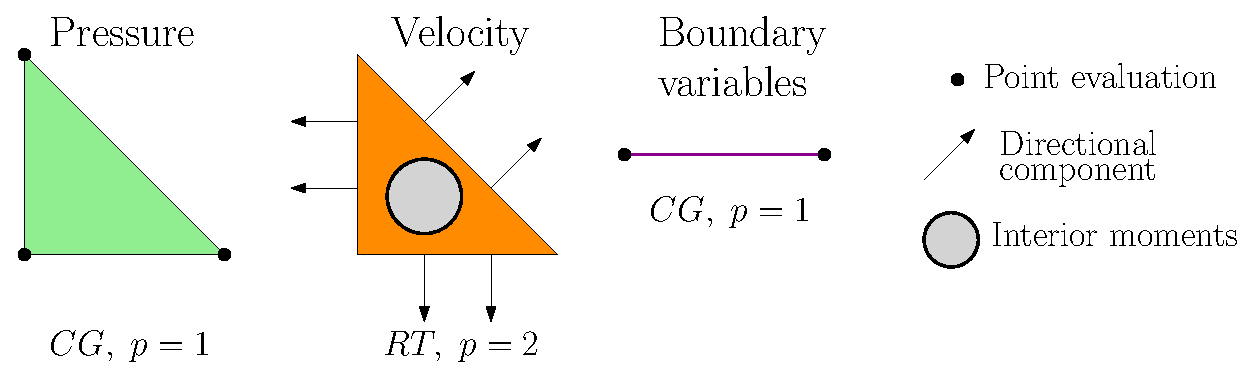
\includegraphics[width=0.9\columnwidth]{fe_sketch.eps}
}

\end{frame}

\begin{frame}[fragile]{Results}

\onslide*<1>{
\begin{figure}[ht]%
	\centering
	\subfloat[][DAE system.]{%
		\label{fig:Htrend_dae}%
		\includegraphics[width=0.48\columnwidth]{Hdae_all.eps}}%
	\hspace{8pt}%
	\subfloat[][ODE system.]{%
		\label{fig:Htrend_ode}%
		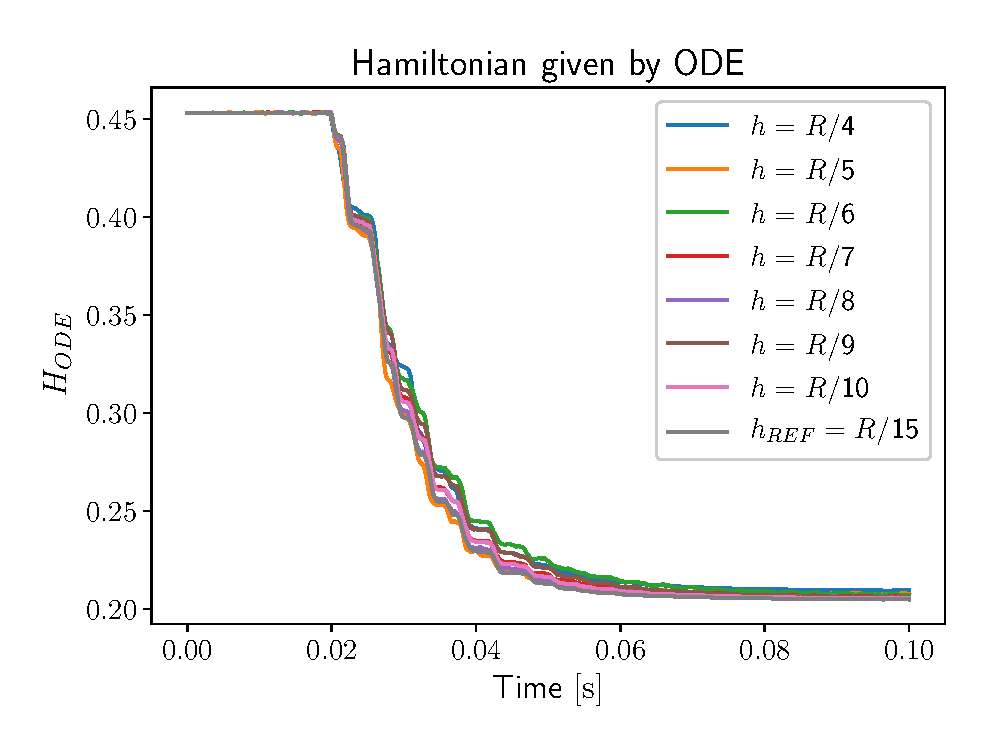
\includegraphics[width=0.48\columnwidth]{Hode_all.eps}} \\
	\caption[]{Hamiltonian trend for different mesh size.}%
\end{figure}
}
\onslide*<2>{
\begin{figure}[ht]%
	\centering
	\subfloat[][Reference Hamiltonian.]{%
		\label{fig:Hdae15}%
		\includegraphics[width=0.48\columnwidth]{Href.eps}}%
	\hspace{8pt}%
	\subfloat[][$L^2$ Hamiltonian error.]{%
		\label{fig:Hdiff}%
		\includegraphics[width=0.48\columnwidth]{Hall_diff.eps}} \\
	\caption[]{Reference Hamiltonian and $L^2$ error.}%
	\label{fig:Href_err}%
\end{figure}
}
\onslide*<3>{
	\begin{figure}[ht]%
		\centering
		\subfloat[][$L^2$ pressure error.]{%
			\label{fig:p_err}%
			\includegraphics[width=0.48\columnwidth]{err_ep.eps}}%
		\hspace{8pt}%
		\subfloat[][$L^2$ velocity error.]{%
			\label{fig:v_err}%
			\includegraphics[width=0.48\columnwidth]{err_eq.eps}} \\
		\caption[]{Error on the state variables for different mesh size.}%
		\label{fig:error_x}%
	\end{figure}
}

\begin{comment}



\begin{center}
\onslide*<4>{
\begin{columns}
\begin{column}{.3\textwidth}
\includemedia[
label=vidNoRod,
addresource=../Videos/wave_dae15.mp4,
activate=pageopen,
width=4cm, height=5cm,
flashvars={
source=../Videos/wave_dae15.mp4
&loop=true
}
]{}{VPlayer.swf}
Reference solution
\end{column}		
\begin{column}{.3\textwidth}
\includemedia[
label=vidNoRod,
addresource=../Videos/wave_dae10.mp4,
activate=pageopen,
width=4cm, height=5cm,
flashvars={
source=../Videos/wave_dae10.mp4
&loop=true
}
]{}{VPlayer.swf}
DAE $h = L/10$
\end{column}
\begin{column}{.3\textwidth}
\includemedia[
label=vidRod,
addresource=../Videos/wave_ode10.mp4,
activate=pageopen,
width=4cm, height=5cm,
flashvars={
source=../Videos/wave_ode10.mp4
&loop=true
}
]{}{VPlayer.swf}
ODE $h = L/10$
\end{column}
\end{columns}	
\mediabutton[
mediacommand=vidNoRod:playPause,
mediacommand=vidRod:playPause
]{\fbox{Play/Pause}}	
%\movie[width=0.8\textwidth, height=0.6\textheight]{Plate and rod}{../Videos/Comparison_RodNoRod.mp4}	
}
\end{center}

\end{comment}

\end{frame}



\begin{frame}{Conclusion}
Future developments:
\begin{itemize}
\item a numerical analysis of the optimal choice for the underlying finite elements \footfullcite{anass2020};
\item  the employment of theses techniques to more complicated models arising from structural and fluid mechanics;
\item reformulation of the approach in terms of differential forms;
\item application of the domain decomposition technique to parallelize simulations of large-scale models.
\end{itemize}
\vspace{1cm}
\centering{\Huge Thanks for your attention} 
\end{frame}

\begin{frame}[allowframebreaks]{References}
\nocite{*}
\printbibliography
\end{frame}

\end{document}
